\documentclass[12pt, twoside]{article}
\usepackage[francais]{babel}
\usepackage[T1]{fontenc}
\usepackage[latin1]{inputenc}
\usepackage[left=7mm, right=7mm, top=7mm, bottom=7mm]{geometry}
\usepackage{float}
\usepackage{graphicx}
\usepackage{array}
\usepackage{multirow}
\usepackage{amsmath,amssymb,mathrsfs}
\usepackage{soul}
\usepackage{textcomp}
\usepackage{eurosym}
 \usepackage{variations}
\usepackage{tabvar}


\pagestyle{empty}

\begin{document}


\section*{\center{Devoir maison 6}}


\bigskip





\fbox{

\begin{minipage}{18cm}
\textit{Devoir � rendre sur feuille grand format petits
carreaux pour le \textbf{lundi 26 avril 2010}.}
\end{minipage}
}

\enskip


 \textit{Remarque: Vous collerez votre �nonc� � la fin de votre copie.
 L'exercice 3 doit �tre lisible une fois la feuille coll�e.}


\bigskip


\ul{Exercice 1}: (\textit{4 points})


\begin{enumerate}
  \item Est-ce-que $\dfrac{7}{3}=2,33$? Expliquer.
  \item Donner l'arrondi au milli�me de $\dfrac{8}{7}$ et la troncature au
  dixi�me de $\dfrac{8}{9}$.
  \item Voici 5 nombres: \qquad 84 \qquad 79 \qquad 501 \qquad 143 \qquad 4950
  
  Lesquels sont divisibles par 2? par 3? par 5? par 9? par 13? 
   Justifier toutes les r�ponses (une r�ponse non justifi�e donnera 0 point).
\end{enumerate}

\bigskip




\ul{Exercice 2}: (\textit{3 points})

\enskip

Pour cet exercice vous d�taillerez toutes les �tapes du calcul et du
raisonnement. Les op�rations seront pos�es � la main sur votre copie.


\begin{enumerate}
  \item L�o a pay� 27,72 \euro pour l'achat de 26,4 litres de carburant. Quel
  est le prix d'un litre de carburant?
  \item Dans une autre station, L�a a achet� pour 27,06 \euro de carburant qui
  co�te 1,10 \euro le litre. Combien de litres de carburant a-t-elle achet�?
\end{enumerate}

\bigskip



\ul{Exercice 3}: \textit{3 points}



\enskip

\begin{center}

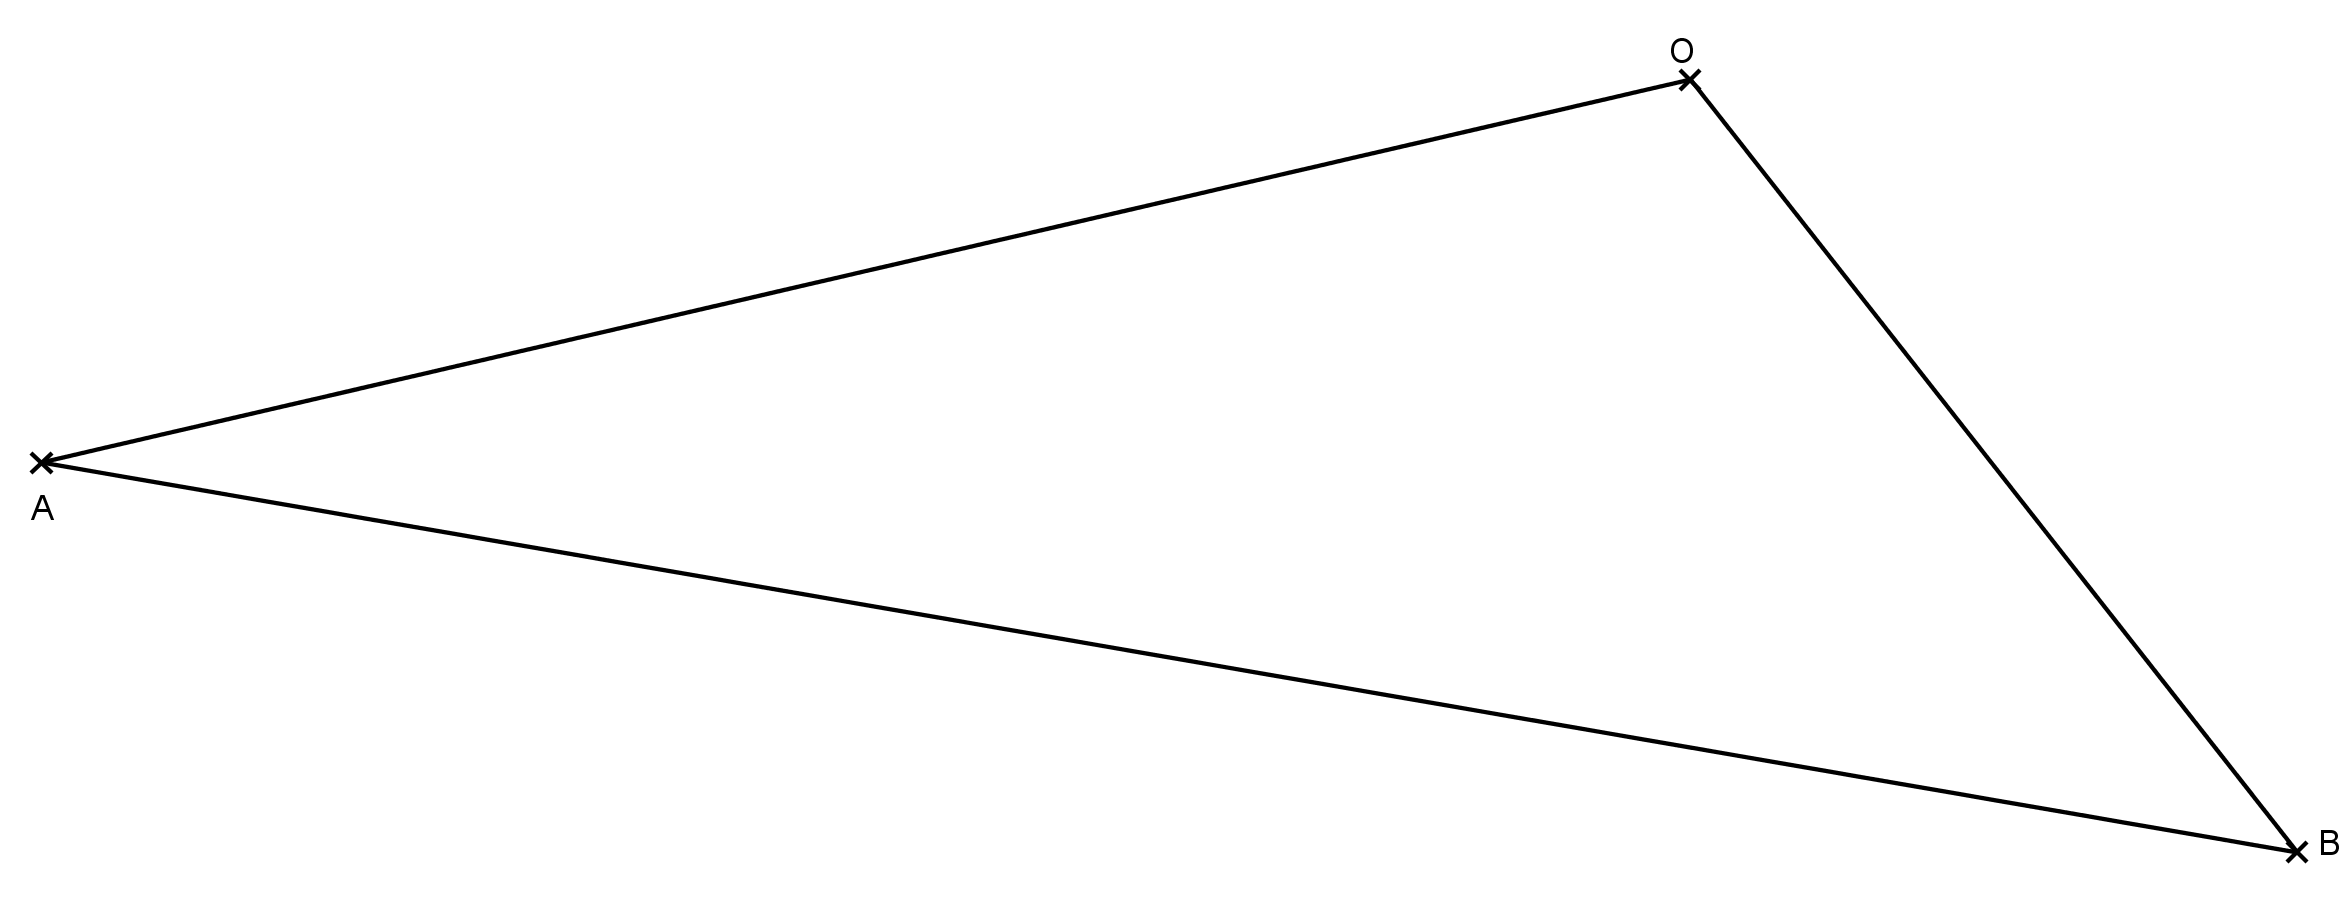
\includegraphics[width=18cm]{images/ex3.png}
\end{center}

\enskip

\begin{enumerate}
\item Tracer en rouge la bissectrice de l'angle $\widehat{ABO}$. On la nomme
$(d_1)$.
\item Tracer en vert la m�diatrice du c�t� [AO]. On la nomme $(d_2)$.
\item Tracer en bleu la m�diane issue de B. On la nomme $(d_3)$.
\item Tracer en noir la hauteur issue de B. On la nomme $(d_4)$.
\item Tracer au crayon gris la m�diane relative au c�t� [OB]. On la nomme
$(d_5)$.
\item Tracer en rouge la hauteur relative au c�t� [AB]. On la nomme $(d_6)$.
\end{enumerate}

Pensez au codage\ldots. 
\end{document}
